% What's the difference between a numerical and theoretical physicists? Physicists are defined in two ways, their area of study and what they produce. Some people argue that numerical is theoretical physics. However, this doesn't sit right with me since we are not on the fundamental behavior of the objects in question. At the same time, experimental physics doesn't feel right either since we are not studying the natural world directly. I think numerical physics is somewhere in between. I believe that are an intermediary. I would say that we are interpreters of theoretical physics, and we run numerical experiments on our computers. 

% I envision this chapter in three broad sections. First,  there is the physics that I use explicitly in this thesis. Secondly, there is the physics that I ignore. Then, there is the implicit physics. Or rather, the physics that I don't build into my experiments explicitly, but emerges naturally arrises from equations of motion. This section thus provides an analytical approach to interpret our results. The second regarding the ignored physics discusses the consequences of ignoring such physics and thus the model limitation. For the physics that I use, I will present simplified cases here that build our interpretation, and then lead to the exact equations of motion that I solve. 

% I will show some solutions explicitly, however, I will discuss the techniques for solving the equations numerically in the next chapter.


\section{The Explicit Physics}
    \subsection*{My equations of Motion} \label{subsec:myEquationsOfMotion}
    \begin{figure}
        \centering
        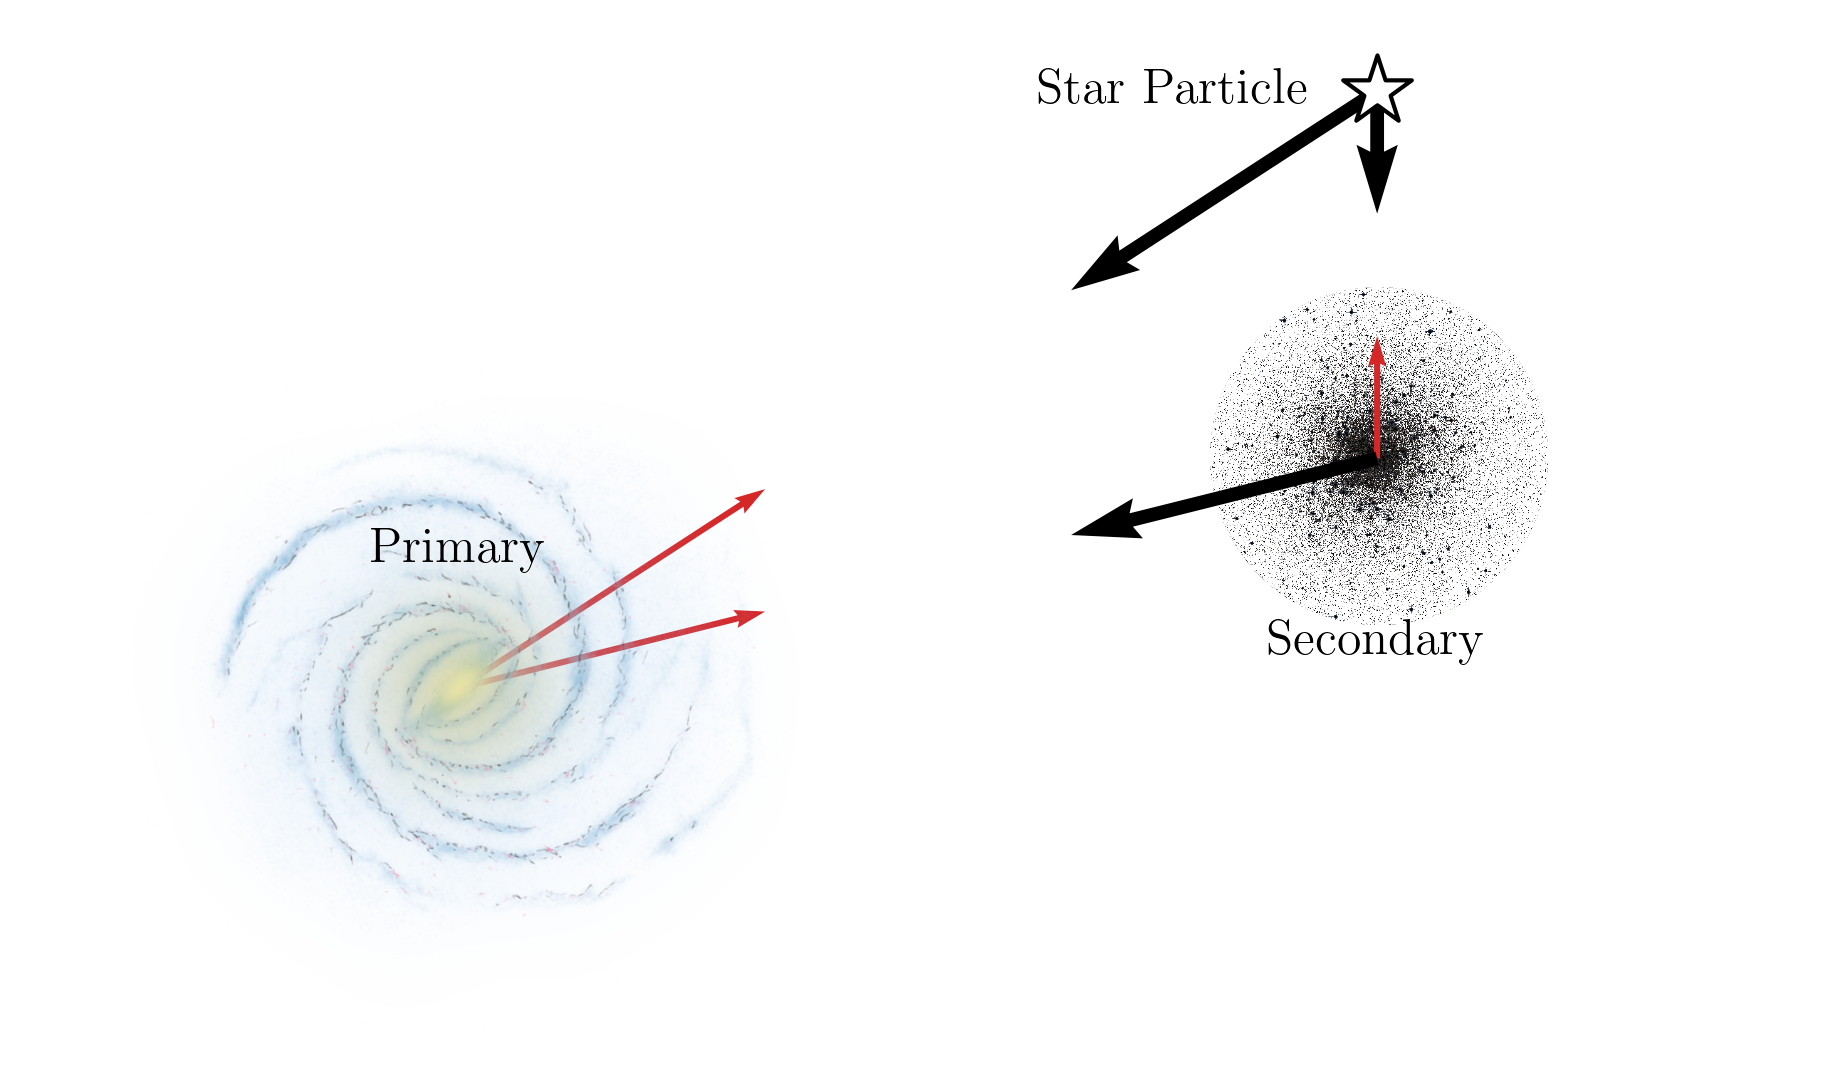
\includegraphics[width=\linewidth]{restricted_three_body_set_up.png}
        \caption{Little sketch of my equations of motion. }
    \end{figure}

    \subsection{Potential density pairs}

        \begin{figure}
            \centering
            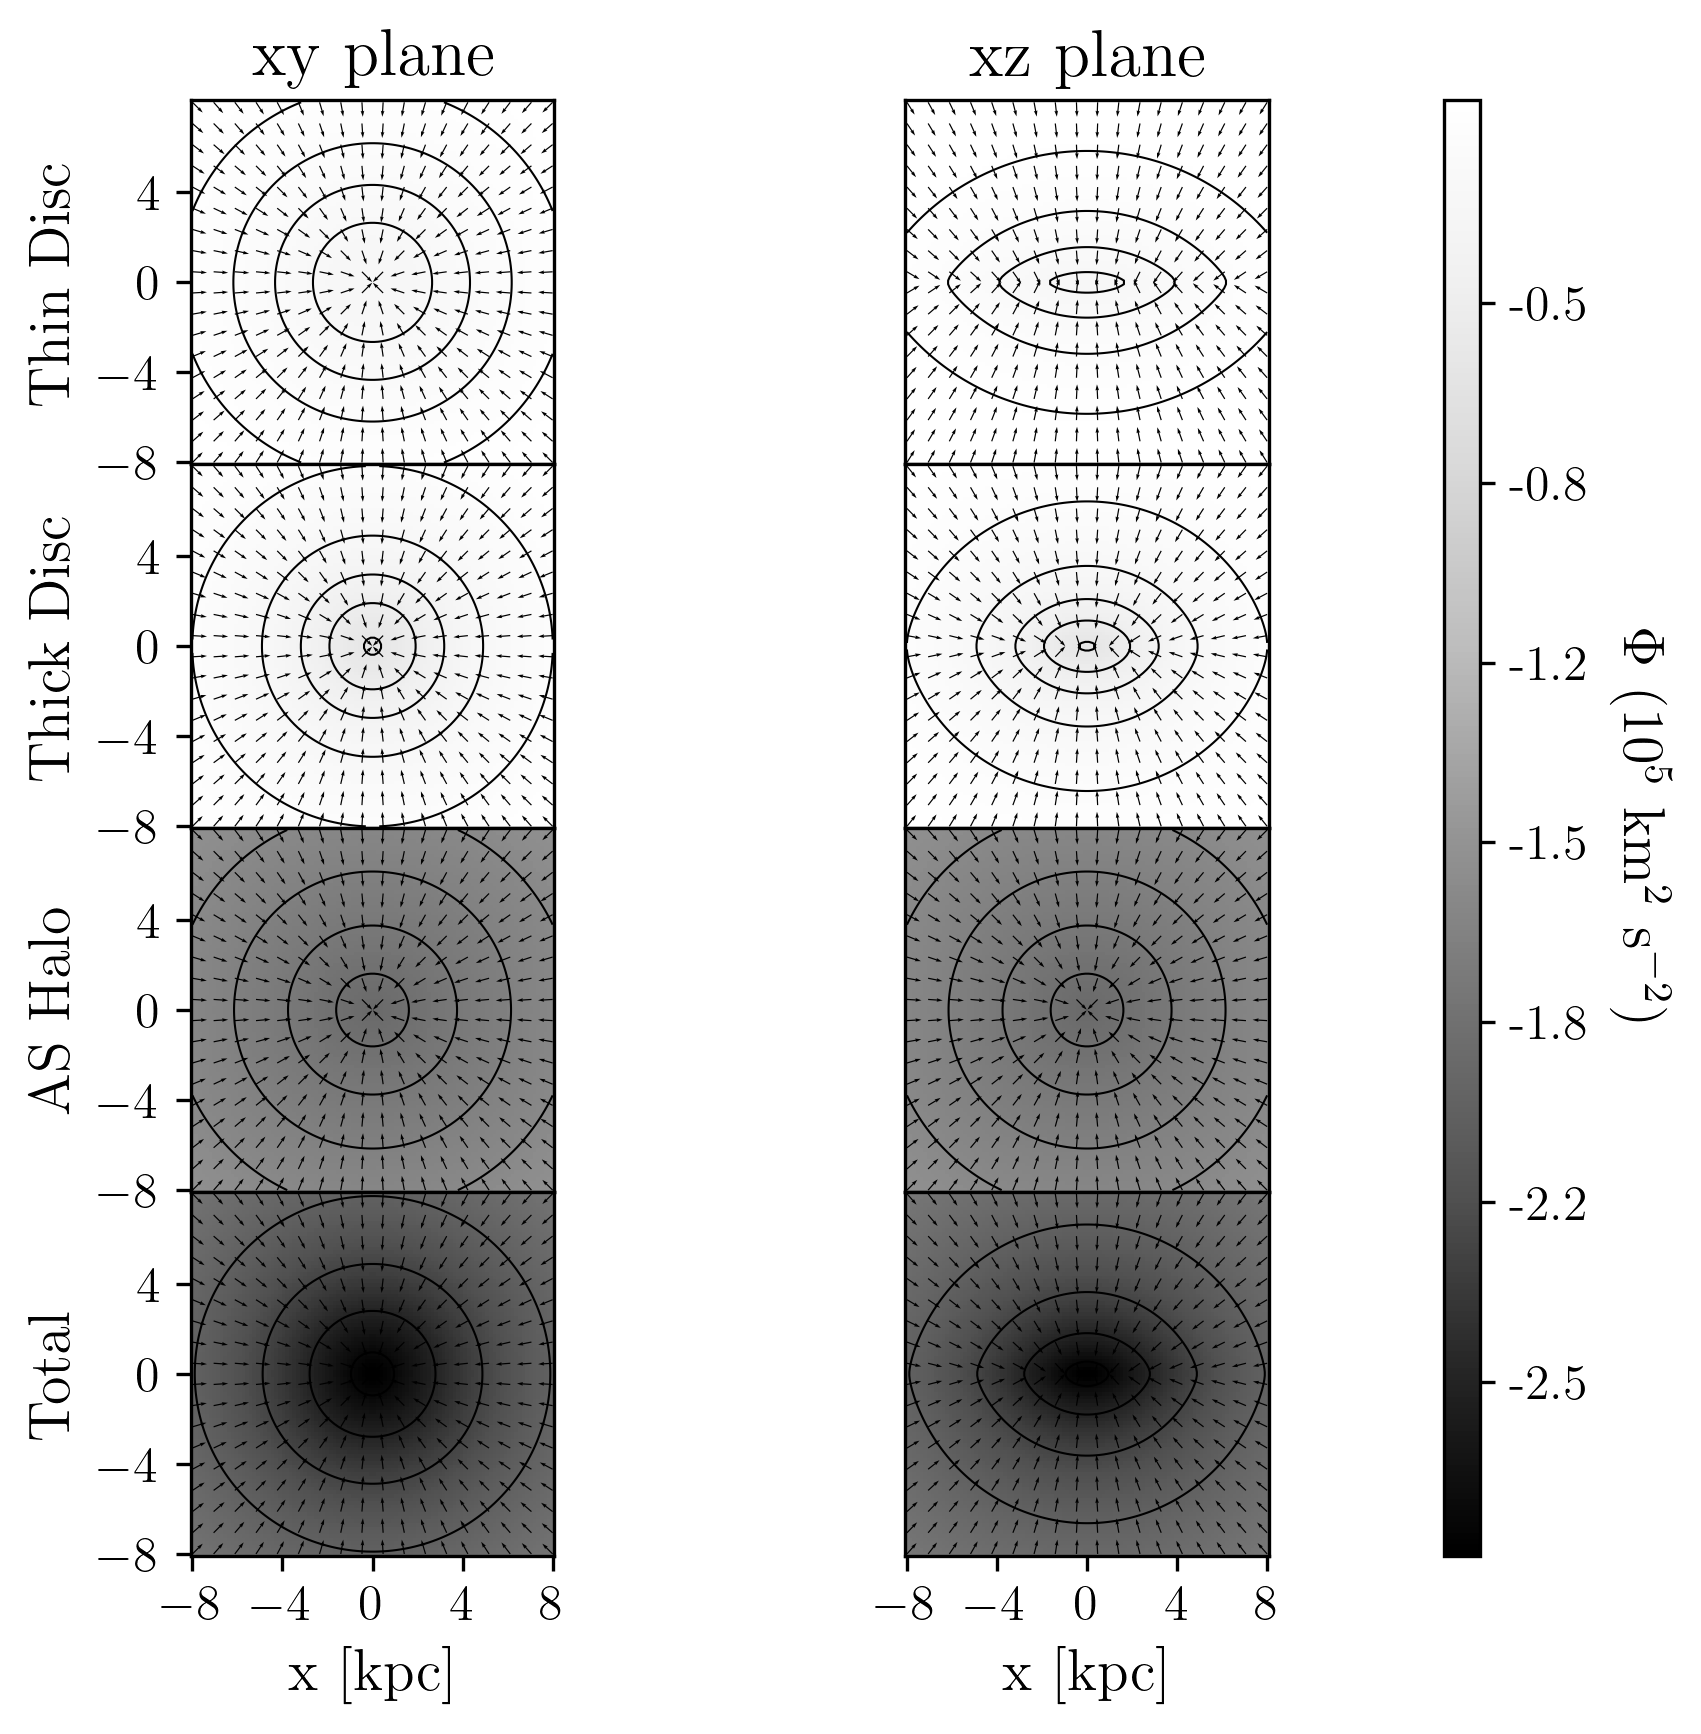
\includegraphics[width=\linewidth]{images/figure_pouliasis2017pii_potential_-8_8.png}
            \caption{nice}
        \end{figure}        
    

\section{The Implicit Physics}

    \subsection{The circular restricted three body problem}

    \subsection{The tidal tensor}
        \begin{itemize}
            \item Show the motivating example of the moon. 
            \item Show the tidal tensor moving around in the case of our galactic potential model 
        \end{itemize}


    \subsection{Phase mixing}
        \begin{itemize}
            \item The Luiville theorem
            \item How it is slower with tidal tails 
            \item also the monte-carlo approach with phase mixing is what causes vast differences in orbital solutions after a certain period of time 
        \end{itemize}
    
    \subsection{Shocks}
        I started this section with the circular and planar restricted three body problem. It really simplifies the problem instead of looking for a general solution. All three bodies are point masses, in fact the tertiary body has no mass. The secondary is on a circular orbit about the primary, and the tertiary is in the same orbital plane as the secondary. This simplified problem is already quite complex but solvable and rich with physics. However, by restricting the orbits of the tertiary and secondary, we lose a lot of physics that affects our system. Additionally, for the globular clustres, most of them are not on circular orbits. Additionally, the galaxy is not a point mass, but rather a mass distribution with cylindrical symmetry.        



\section{The Ignored Physics}
    \subsection{Collisional dynamics}
        \begin{itemize}
            \item not nbody
            \item no mass segregation
            \item no three body encounters 
            \item no soft or hard binaries 
            \item show some results from Corespray 
        \end{itemize}
    
    \subsection{Stellar evolution}
        \begin{itemize}
            \item They're all point masses 
            \item No salpeter's 
            \item No strong initial mass loss 
            \item No accurate model for the colors 
            \item No multiple stellar populations 
        \end{itemize}
    
    \subsection{Time evolution}
        In someways, we take time evolution into account, and in someways, we ignore and this has already been covered in the previous sections. i.e., the orbit of the star-particles depend on the position of the host globular cluster, which I do not solve for simoltaneously but instead opt to load it into the computation, as shown in Section~\ref{subsec:myEquationsOfMotion}. Also, things like mass segregation and stellar evolution are time-dependent which is completely ignored in my simulations. 

